\section{Visual Studio 2022}
\setauthor{Mirzet sakonjic}
\cite{VS2022}
\begin{figure}[h]
    \begin{center}
        \includegraphics*[width=6cm]{pics/Visual-Studio-Logo.png}
        \caption[VS 2022 Logo]{Visual Studio 2022 Logo \cite{VS2022logo}}
    \end{center}
\end{figure}
\subsection*{Erklärung}
Visual Studio Enterprise 2022 ist eine integrierte Entwicklungsumgebung für verschiedene Hochsprachen von Microsoft welche im Jahr 2022 (Juni) veröffentlicht wurde.
Visual Studio ermöglicht es Programmierern, sowohl Win32/Win64-Programme als
auch Anwendungen für das .NET Framework zu entwickeln. Darüber hinaus lassen sich
mit Visual Studio Windows-Apps, dynamische Webseiten bzw. Webservices für das
Internet/Intranet oder Azure-Services entwickeln.
\subsection*{Funktionalität}
Visual Studio ist eine sehr umfangreiche und komfortable Entwicklungsumgebung. Sie
lässt sich gezielt auf die Anforderungen von Projekten anpassen. Mit dem VS-Installer
können zusätzliche Hochsprachen installiert oder deinstalliert werden.
Neben der Erweiterbarkeit stellt Visual Studio einen integrierten Debugger zur Verfügung. Dieser enthält die Funktion „Bearbeiten und Fortfahren“ und erlaubt das
nachträgliche Anhängen an bereits laufende Prozesse, sowohl am lokalen Rechner als
auch über das Netzwerk. Neben dem Debugger wird der Softwareentwickler durch eine
gute IntelliSense unterstützt.
\subsection*{Begründung und Verwendung}
Visual Studio ist die etablierteste Entwicklungsumgebung auf dem Markt, um .NET
zu programmieren, da es sich durch seinen Umfang und die gute Bedienbarkeit ausgezeichnet. Aufgrund der vielen Funktion, der Marktposition und der Tatsache, dass
sich Visual Studio bereits in vergangenen Projekten bewährt hat, wurde es für unsere
Arbeit gewählt. Die Enterprise Lizenz wurde von der HTL zur Verfügung gestellt und
darf ausschließlich für schulische Zwecke eingesetzt werden.
\newpage

\section{Visual Studio Code}
\setauthor{Stefano Pyringer}

% Bilder sollten nebeneinander sein
\begin{figure}[htb]
    \begin{center}
        
\includegraphics[width=3cm] {./pics/Visual_Studio_Code_1.35_icon.svg.png}
        \caption{Visual Studio Code Logo}
        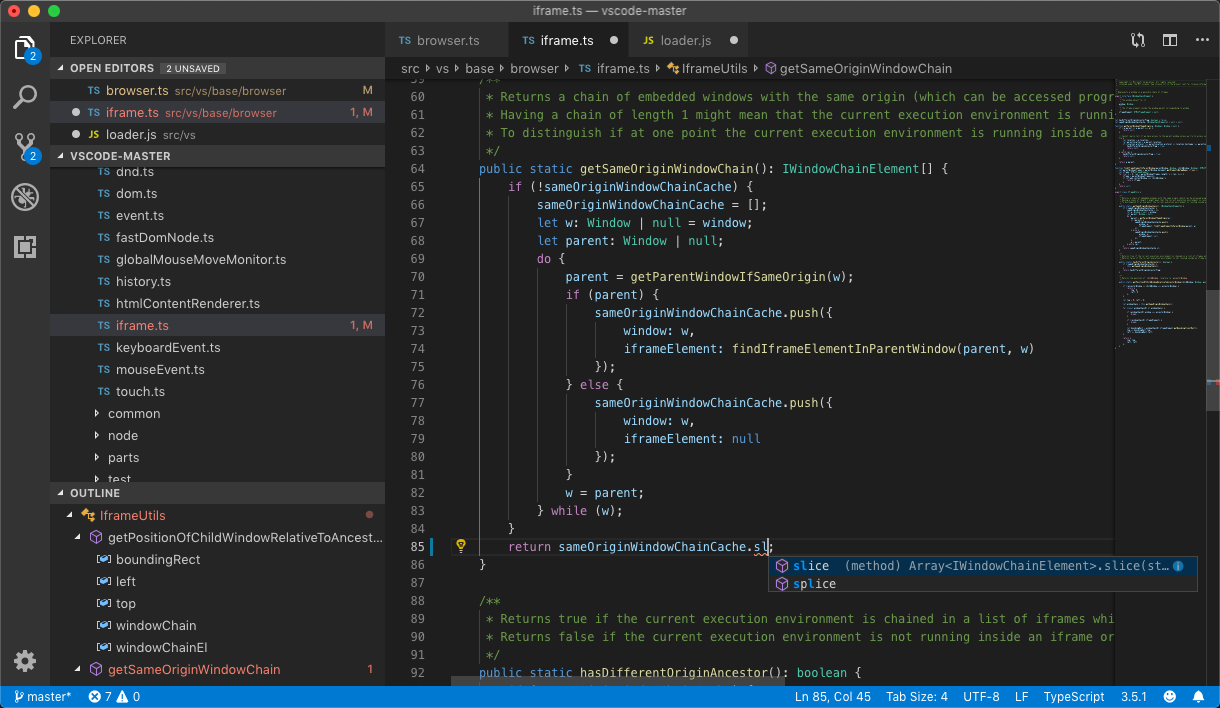
\includegraphics[width=6cm]{./pics/VS_Code_1.36.0-insider.png}
        \caption{Visual Studio Code Screenshot}
    \end{center}
\end{figure}

Visual Studio Code, wird auch als VS Code bezeichnet, ist ein Code-Editor entwickelt von Microsoft. 
Seit November 2015 ist der Source-Code des Code-Editors auf Github verfügbar. Im April 2016 wurde die erste finale Version 
von Visual Studio Code veröffentlicht. Der Source-Code des Code-Editors ist mit einer MIT-Lizenz lizensiert und ist somit Open-Source.
Das installierbare Programm hingegen enthält Microsoft-Binaries und ist deshalb keine Open-Source. Das Programm ist kostenlos verfügbar.

Der Texteditor basiert auf dem App-Framework Electron und läuft daher in der Chromium-Engine. Standardmäßig werden ohne zusätzliche Instalationen
die gängigen Programmier- und Scriptsprachen wie HTML, JavaScript, SQL, JSON, C, etc. unterstützt. 
Folgende Basisfunktionen besitzt das Entwickler-Tool:

\begin{itemize}
    \item Syntaxhervorhebung
    \item Autovervollständigung
    \item Code-Folding % (ev. Erklärung Fusszeile!)
    \item Debugging
    \item Versionsverwaltung
    \item Konfigurierbare Code-Snippets
    \item IntelliSense für TypeScript, JSON, CSS und HTML
    \item Extension-Support
\end{itemize}

\subsection{Unterschiede zu Visual Studio}
\setauthor{Stefano Pyringer}
Entwicklungsumgebungen (IDEs) wie Visual Studio sind meistens für ein Betriebssystem entwickelt worden und funktionieren 
gar nicht oder nur eingeschränkt auf anderen Betriebssystemen. Die Auswahl von Programmiersprachen und Frameworks ist beschränkt. IDEs 
haben üblicherweise einen hohen Speicher- und Ressourcenbedarf.

Visual Studio Code hingegen ist ein Texteditor, der in der Chromium-Engine läuft und ist für alle 3 gängigen Betriebssysteme 
Windows, MacOs und Linux verfügbar. Aufgrund des niedrigen Ressourcenbedarfs ist es auch auf schwächeren oder älteren Computern und Laptops benutzbar.
Ein großer Unterschied zu Visual Studio ist die Dateiveraltung. 
In Entwicklungsumgebungen wird ein Projekt in Projektdateien zusammengefasst, 
währendessen der Code-Editor mit Workspaces arbeitet. Diese speichern den 
Bearbeitungszustand, Reihenfolge und Zeilenposition der geöffneten Dateien. 
In Visual Studio Code wird ein Workspace geöffnet, indem ein Ordner ausgewählt wird.

Ein Texteditor kann den Funktionsumfang und Komfort einer Entwicklungsumgebung nicht mithalten. Visual Studio Code 
kann dank Plug-ins, werden auch als Extensions bezeichnet, in der Funktionalität stark erweitert werden.
Ein großer Vorteil zu Visual Studio ist der Extension-Marketplace, die von einer großen Gemeinschaft von Entwicklern gepflegt wird.
Dank einer Vielzahl von Plug-ins ist fast jede beliebige Sprache mit umfangreichen Hilfsfunktionen wie IntelliSense oder Snippets verfügbar.

\subsection{Verwendungsgrund}
\setauthor{Stefano Pyringer}
Visual Studio Code wurde für dieses Projekt für die Testung der HTML-Schnittstellen (APIs) des Programms und für die Planung der Datenbankobjekte verwendet.
Es wurden im Unterricht bereits gute Erfahrungen mit dem Code-Editor gemacht. Ein großer Vorteil ist der sparsame Verbrauch von Ressourcen, 
da das Projekt großteils mit Laptops entwickelt wurde und der große Funktionsumfang von bekannten Entwicklerwerkzeugen nicht benötigt wurde.

Es wurden folgende Plug-ins verwendet:
\begin{itemize}
    \item Thunder Client
    \item ERD Editor
\end{itemize}

% Link zu Extension einfügen?
\subsection{Thunder Client Extension}
\setauthor{Stefano Pyringer}
Die Thunder Client Extension ist eine leichtgewichte REST-API, die sich durch eine einfach zu bedienende GUI auszeichnet.
Sie unterstützt API Collections, Environment Variablen und kommt auch mit großen Anfragen klar. Desweiteren können die API Anfragen 
ohne Script mithilfe der GUI getestet werden. Sie ist eine schnelle und einfache Alternative zu Postman.

% Link zu Extension einfügen?
\subsection{ERD Editor Extension}
\setauthor{Stefano Pyringer}
Der ERD Editor ist eine Extension für Visual Studio Code, mit der die Planung von Datenbankobjekten und deren 
Beziehungen ermöglicht wird. Mithilfe dieses Plug-ins sind verschiedene grafische Darstellungen des Entity Relation Diagramms möglich.
Ein Code-Generator kann die geplanten Datenbankobjekte in SQL-DDL-Code umwandeln. Die Extension ist eine Alternative zu Planungswerkzeugen, 
die z. B. im Oracle SQL Developer enthalten sind.
\newpage

\section{Github}
\setauthor{Mirzet Sakonjic}
\cite{GitHub}
\begin{figure}[h]
    \begin{center}
        \includegraphics*[width=8cm]{pics/GitHub_Logo.png}
        \caption[GitHub Logo]{GitHub Logo \cite{GithubLogo}}
    \end{center}
\end{figure}
\subsection*{Erklärung}
GitHub ist die primäre Plattform für Entwickler, um ihre Software zu hosten 
und zu verwalten. wurde 2008 gegründet und 2018 von Microsoft gekauft. 
Da GitHub dennoch zu einer wichtigen Anlaufstelle geworden ist, 
kann es in dieser Weise lange Zeit als soziales Netzwerk für Entwickler 
verstanden werden. Jeder hat dort sein eigenes Profil, einige arbeiten 
nur an Open-Source-Software und werden von Sendeanstalten finanziert. 
Andere führen ihre privaten Projekte nach der Arbeit durch oder unterstützen 
größere Projekte nur zum Spaß.
\subsection*{Funktionalität}
Um ein Programm, eine Website oder ähnliches bearbeiten oder durchsuchen zu können, 
muss das Repository oder Verzeichnis öffentlich sein oder Sie müssen dazu eingeladen 
werden. Und wenn dies nicht der Fall ist, kann nur der Ersteller des Repositorys 
daran arbeiten. An einem Verzeichnis können beliebig viele Entwickler arbeiten. 
Um einen Beitrag leisten zu können, müssen Sie das Repository forken, was bedeutet, 
dass Sie eine Kopie auf Ihrem eigenen Konto mit den aktuellen Daten erstellen. 
Wenn der Ersteller des ursprünglichen Repositorys dies später zulässt, können die 
beiden Repositorys wieder zusammengeführt werden. Dies wird als Zusammenführen 
bezeichnet. Sie können auch einfach dem Repository oder Entwickler folgen. 
GitHub wird von Microsoft betreuet.
\subsection*{Begründung und Verwendung}
GitHub ist die seriöseste und bekannteste Plattform auf dem Markt für Teamprojekte 
und -arbeiten, da sie sich durch Geschwindigkeit und Benutzerfreundlichkeit 
auszeichnet. Es wurde aufgrund seiner zahlreichen Funktionen und der Kompatibilität 
mit Visual Studio für unsere Arbeit ausgewählt. Es gibt keine Lizenz und es kann 
kostenlos für jeden Zweck verwendet werden.
\newpage

\section{Testen auf dem Endgerät}
\subsection{Android Emulator}
\newpage

\subsection{iOS Emulator}
\setauthor{Mirzet Sakonjic}
\cite{IOsEmulatorOnMac}
\cite{IOsEmulatorOnWin}
\subsubsection*{Erklärung}
Der Emulator kann in andersartigen Konfigurationen 
ausgeführt werden, um andersartige Apparate zu schauspielern. 
Jede Justierung wird als virtuelles Endgerät bezeichnet. 
Wenn Sie Ihre Application auf einem Emulator bereitstellen 
und prüfen, wählen Sie ein vorkonfiguriertes oder 
benutzerdefiniertes virtuelles Device aus, das ein 
physisches iOS-Gerät wie ein iPhone-Telefon simuliert.
\subsubsection*{Funktionalität}
Mit dem Remote-iOS-Simulator für Windows können Sie Ihre 
Applikationen auf einem iOS-Simulator prüfen, der unter Windows mit 
Visual Studio 2022 angezeigt wird.
Der Remote-iOS-Simulator für Windows wird von selbst als Teil der 
Arbeitsauslastung der plattformübergreifenden .NET-Anwendungs-UI-Entwicklung 
in Visual Studio 2022 eingerichtet. Die Einrichtung besteht aus einigen Schritten.
Mit Xamarin.Mac können Sie ohne Ausnahme native Mac-Anwendungen in C-Sharp und .NET 
erzeugen. Da Xamarin.Mac schnell in Xcode eingebettet ist, können 
Entwickler den Interface Builder von Xcode verwenden, um Anwendungsbenutzeroberflächen 
zu anlegen (optional kann dies genauso einfach in C-Sharp-Code erfolgen). 
Auf jene Weise war es ausgeprägt schneller, problemloser und effektiver, 
die iOS-Anwendung durch des Apple-Betriebssystems zu prüfen.
\subsubsection*{Begründung und Verwendung}
Xamarin iOS Emulator ist für das Testen mobiler Applikationen unverzichtbar, 
da es längst als Teil der Xamarin-Plattform eingerichtet ist. Das Testen 
geschieht gleichzeitig, was es außergewöhnlich nützlich macht. 
Wir haben uns für den iOs-Emulator entschieden, weil es wahrscheinlich 
ist, auf zwei differenzierten Plattformen (Windows und iOs) zu 
begutachten. Es existieren keine Lizenz, trotz alledem es ist Teil der Xamarin-Plattform.
\newpage